\section*{Figure Captions}
\renewcommand\thefigure{}
%\renewcommand*{\figureformat}{\figurename~}{}
\newcommand\fnum[1]{\textbf{\ref{fig:#1}.} }
%
\begin{figure*}[!hb]
\centering
\hide{
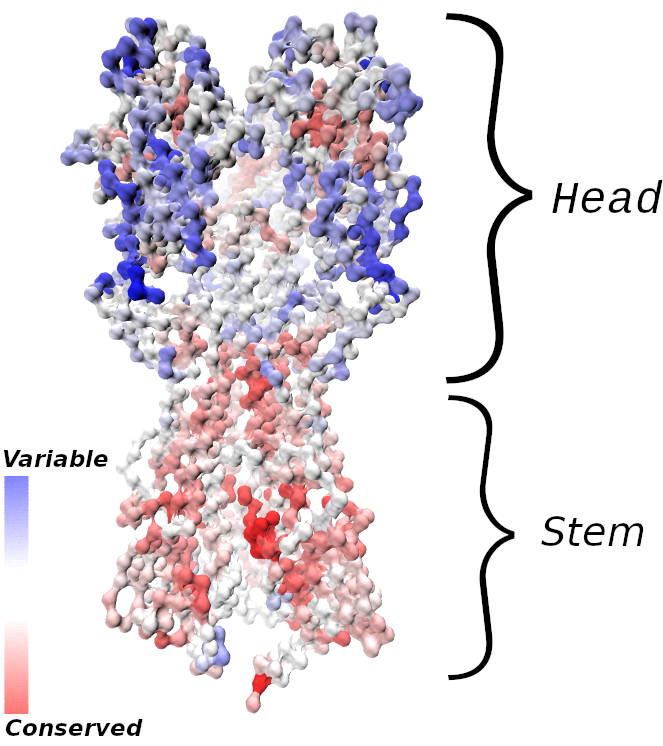
\includegraphics[width=0.4\textwidth]{cons3i.png}
}
\caption{\fnum{cons}
Influenza hemagglutinin (HA) spike protein colored by residue conservation. Sequences of avian, swine and human influenza type A 
spike proteins were downloaded from the NIH influenza research database\cite{bao08}; conservation was computed in MATLAB\cite{matlab} after
clustering the sequences to 97\%~identity and multiple alignment. The HA structure was taken from PDB entry 3LZG\cite{xu10}, and the image was generated
using Visual Molecular Dynamics.\cite{Humphrey96} Only the $C_\alpha$ atoms are shown.
}
%\label{fig:cons}
\end{figure*}
%
\begin{figure}[hb]
\centering
\hide{
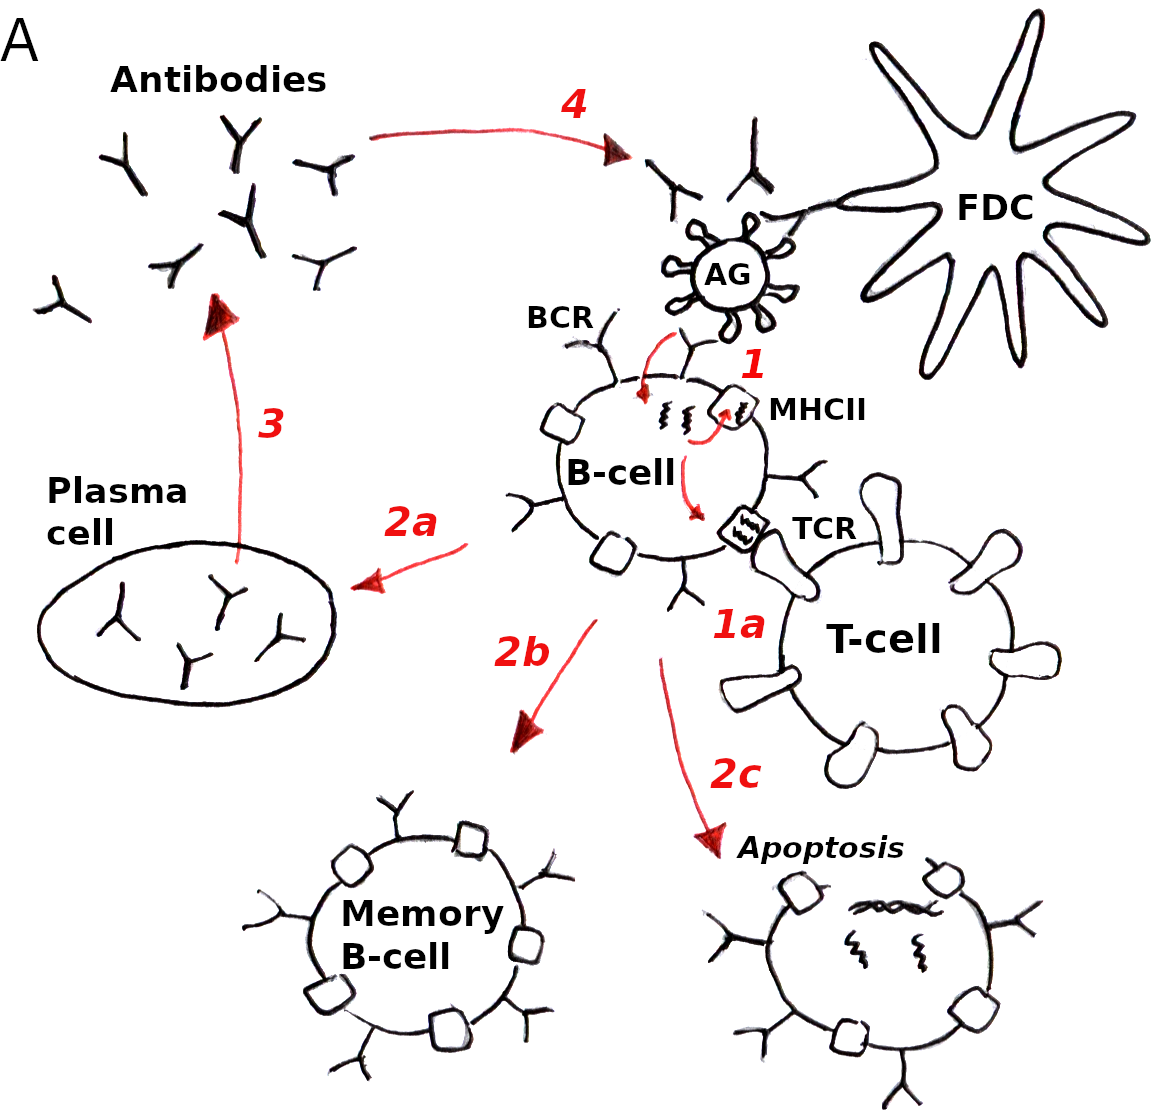
\includegraphics[width=0.43\textwidth,valign=t]{model2i.png}
\hspace{2EM}
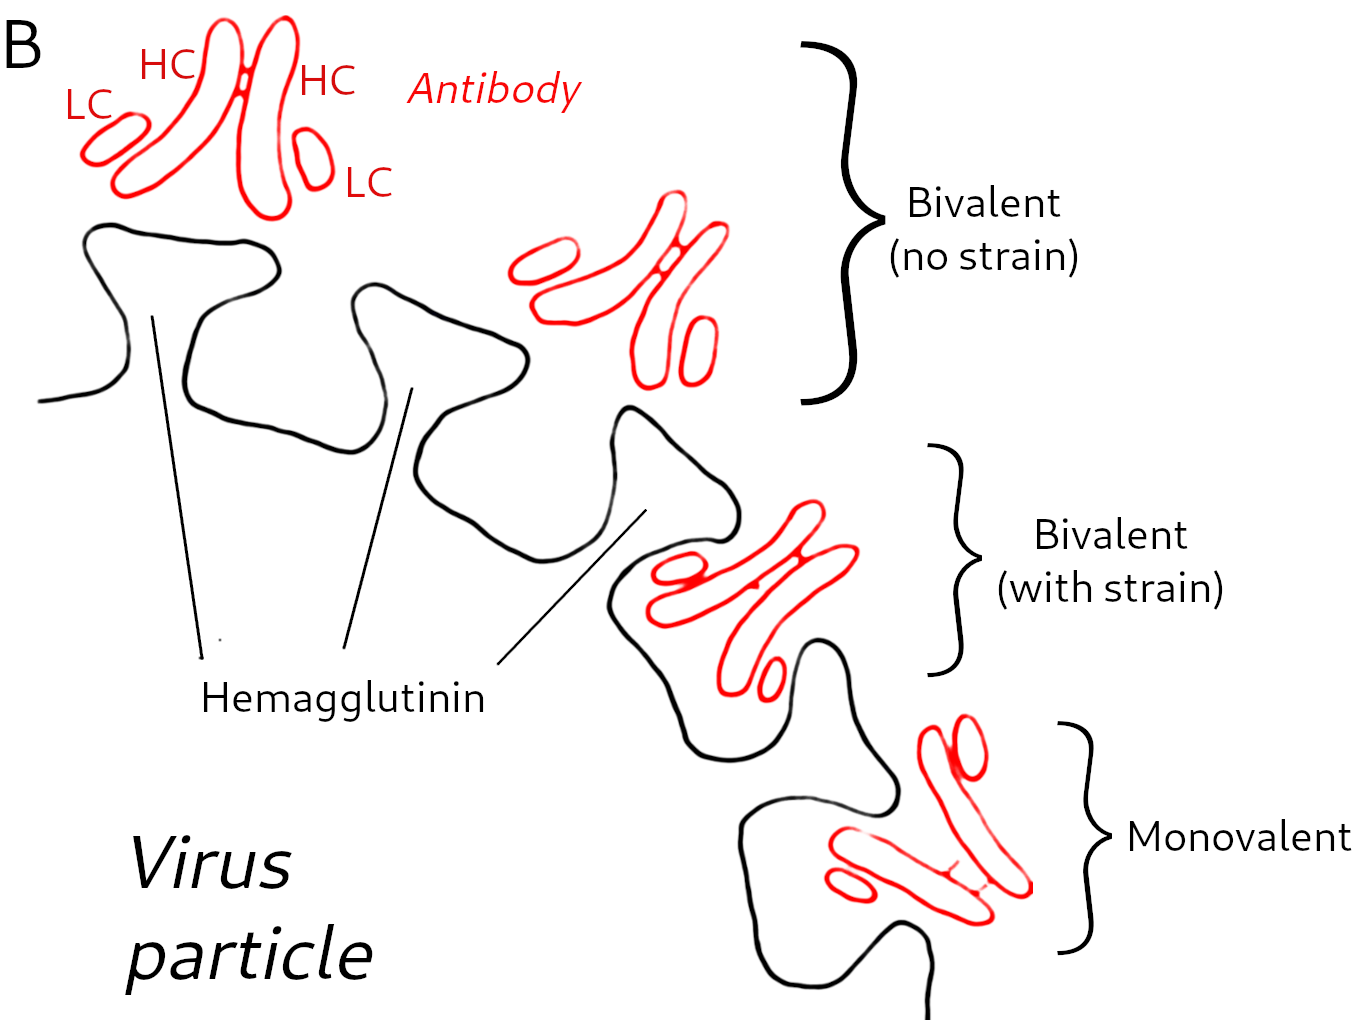
\includegraphics[width=0.49\textwidth,valign=t]{ab-ha-avidity3.png}
}
\caption{\fnum{model}Schematic of the GC model used in this study. (A) Model overview: (1) B-cells are activated upon binding to antigen presented on
follicular dendritic cells (FDCs, not explicitly modeled); (1a) in the optional T-cell help model (see text) B-cells are
activated when the major histocompatibility complex receptor (MHC2) binds to the T-cell receptor (TCR); B-cell activation rescues
B-cells from apoptosis, allowing them to mutate and proliferate; (2) depending on the activation signal,
B-cells can differentiate to plasma cells (2a), to memory B-cells (2b), or undergo apoptosis (2c); (3) Plasma cells secrete antibodies
(Abs), which also compete with B-cell receptors for antigen (4), which is the essential aspect of the Ab feedback model\cite{zhang13}
(see text). (B) Hypothetical modes of antibody binding to influenza spikes; bivalent binding without strain (top) corresponds to
cooperative binding by antibody arms; bivalent binding with strain (middle) corresponds to noncooperative binding; monovalent binding (bottom) is assumed to be the
dominant mode of binding of anti-HA stem antibodies (see Methods for details).
}
%\label{fig:model}
\end{figure}
%
\begin{figure*}[hb]
\centering
\hide{
\includegraphics[width=0.32\textwidth]{basetest3x-valid-gcsize.eps}
\includegraphics[width=0.32\textwidth]{basetest3x-valid-dmbc.eps}
\includegraphics[width=0.32\textwidth]{basetest3x-valid-dplc.eps}
}
\caption{\fnum{valid}Comparison of simulation and experiments.
A: Total B-cells, B: Memory B-cell production rate, C: Plasma cell
production rate. Experimental data for panel A was generated from the GC
cross-sectional areas plotted in Fig.~S1B of Ref.~\citenum{wittenbrink11}, and converted to B cell counts
as done in Ref.~\citenum{pelissier20}; \vo{The lower and upper error bars in panel A
corresponds to 30\%~and 70\%~quantiles, respectively}
; experimental data for panels B \& C was taken from Fig.~4 of Ref.~\citenum{pelissier20}, who
obtained raw data from \citet{weisel16}; \vo{the error bars in B \& C correspond to approximately one SD.}
}
%\label{fig:valid}
\end{figure*}
%
\begin{figure*}[hb]
\centering
\hide{
\includegraphics[width=0.49\textwidth]{basetest3x-o0-gcsize.eps}
\includegraphics[width=0.49\textwidth]{basetest3x-o1-gcsize.eps}
\includegraphics[width=0.49\textwidth]{basetest3x-o0-dmbc.eps}
\includegraphics[width=0.49\textwidth]{basetest3x-o1-dmbc.eps}
\includegraphics[width=0.49\textwidth]{basetest3x-o0-A.eps}
\includegraphics[width=0.49\textwidth]{basetest3x-o1-A.eps}
}
\caption{\fnum{avidity}Effect of antibody valency and epitope occlusion on GC properties.
Left column (A--C): noninteracting B-cell case ($o=0$);
Right column (D--F): fully interacting B-cell case ($o=1$);
A,D: Total B cells;
B,E: Memory cell production rate; insets: total MBC population at end of simulation;
C,F: Average affinity of B-cells and MBCs.  For the definition of occlusion $o$, see \sec{occlusion}.
}
%\label{fig:avidity}
\end{figure*}
%
\begin{figure*}[hb]
\centering
\hide{
\includegraphics[width=0.5\textwidth]{basetest3x-o1x7-gcsize.eps}
\includegraphics[width=0.49\textwidth]{basetest3x-o1x7-dmbc.eps}
\includegraphics[width=0.5\textwidth]{basetest3x-o1x7-A.eps}
\includegraphics[width=0.49\textwidth]{basetest3x-o1x7-dist.eps}
}
\caption{\fnum{kadv}Effect of initial affinity advantage on the growth of monovalent B-cells in the fully interacting B-cell case ($o=1$).
Panels A--C show the same quantities as \fig{avidity}A--C;
The affinity distribution corresponding to BCR\#1 was shifted toward higher values relative to BCR\#2 and BCR\#3
(panel D).
}
%\label{fig:kadv}
\end{figure*}
%
\begin{figure*}[hb]
\centering
\hide{
\includegraphics[width=0.99\textwidth]{test5ki-d3x-occl-k12=10agc1=1.eps}
\includegraphics[width=0.99\textwidth]{test5ki-d3x-occl-k12=0agc1=1.eps}
}
\caption{\fnum{kadv2}Fraction of MBC\#1 ($\zeta$, \vo{defined in the text}) at the end of six GC simulations for different initial affinity advantage values
 \vs~total number of BCR/Epitope pairs.
A: BCR\#1 is cooperatively bivalent ($K^{12}_{eq}$=10$K^{11}_{eq}$);
B: BCR\#1 is monovalent ($K^{12}_{eq}$=0).
}
%\label{fig:kadv2}
\end{figure*}
%
\begin{figure}[hb]
\centering
\hide{
\includegraphics[width=0.49\textwidth]{basetest3x-o1-a1-2-gcsize.eps}
\includegraphics[width=0.49\textwidth]{basetest3x-o1-a1-2-dmbc.eps}
\includegraphics[width=0.49\textwidth]{basetest3x-o1-a1-2-A.eps}
}
\caption{\fnum{agc1}Effect of BCR valency and epitope concentration on GC evolution, with $o=1$ (fully competitive case).
Panels A--C show the same quantities as \fig{avidity}A--C;
$\alpha_1^T=2$, $\alpha_2^T=1$, $\alpha_3^T=1$; $\alpha^T$ is the nondimensional AG concentration (see \sec{integration}).
}
%\label{fig:agc1}
\end{figure}
%
\begin{figure*}[!ht]
\centering
\hide{
\includegraphics[width=0.99\textwidth]{test5kj-d3x-mbctime-k12=10.eps}
\includegraphics[width=0.99\textwidth]{test5kj-d3x-mbctime-k12=0.eps}
}
\caption{\fnum{agtime}Fraction of MBC\#1 \vs~number of sequential GC simulations for different initial affinity advantage values
and different AG\#1 concentrations, with 10 total BCR/Epitope pairs.
A \& B: MBC\#1 fraction ($\zeta$) at the end of simulations.
A: BCR\#1 is cooperatively bivalent ($K^{12}_{eq}$=10$K^{11}_{eq}$);
B: BCR\#1 is monovalent ($K^{12}_{eq}$=0).  
The four sets of panels A and B show the effect of increasing occlusion from $o$=0 (no
competition) to $o$=1 (full competition).
}
%\label{fig:agtime}
\end{figure*}
